\documentclass[a4paper,12pt]{article}
\usepackage{amsmath,amssymb}
\usepackage{graphicx}
\usepackage{scaladefs}
\usepackage{scalit}
\usepackage{fancyhdr}
\pagestyle{fancy}
\lhead{\today}
\rhead{weave/weave.nw}
\begin{document}
\section{Weave - Creating documentation out of a literate program}
The program described here allows us to extract a human readable file
out of the \texttt{noweb} input. The content will be output in the order that
it was written in the noweb file, but code sections will be annotated and
we will gather information that allows us to indicate information like
which class was defined where and so on.

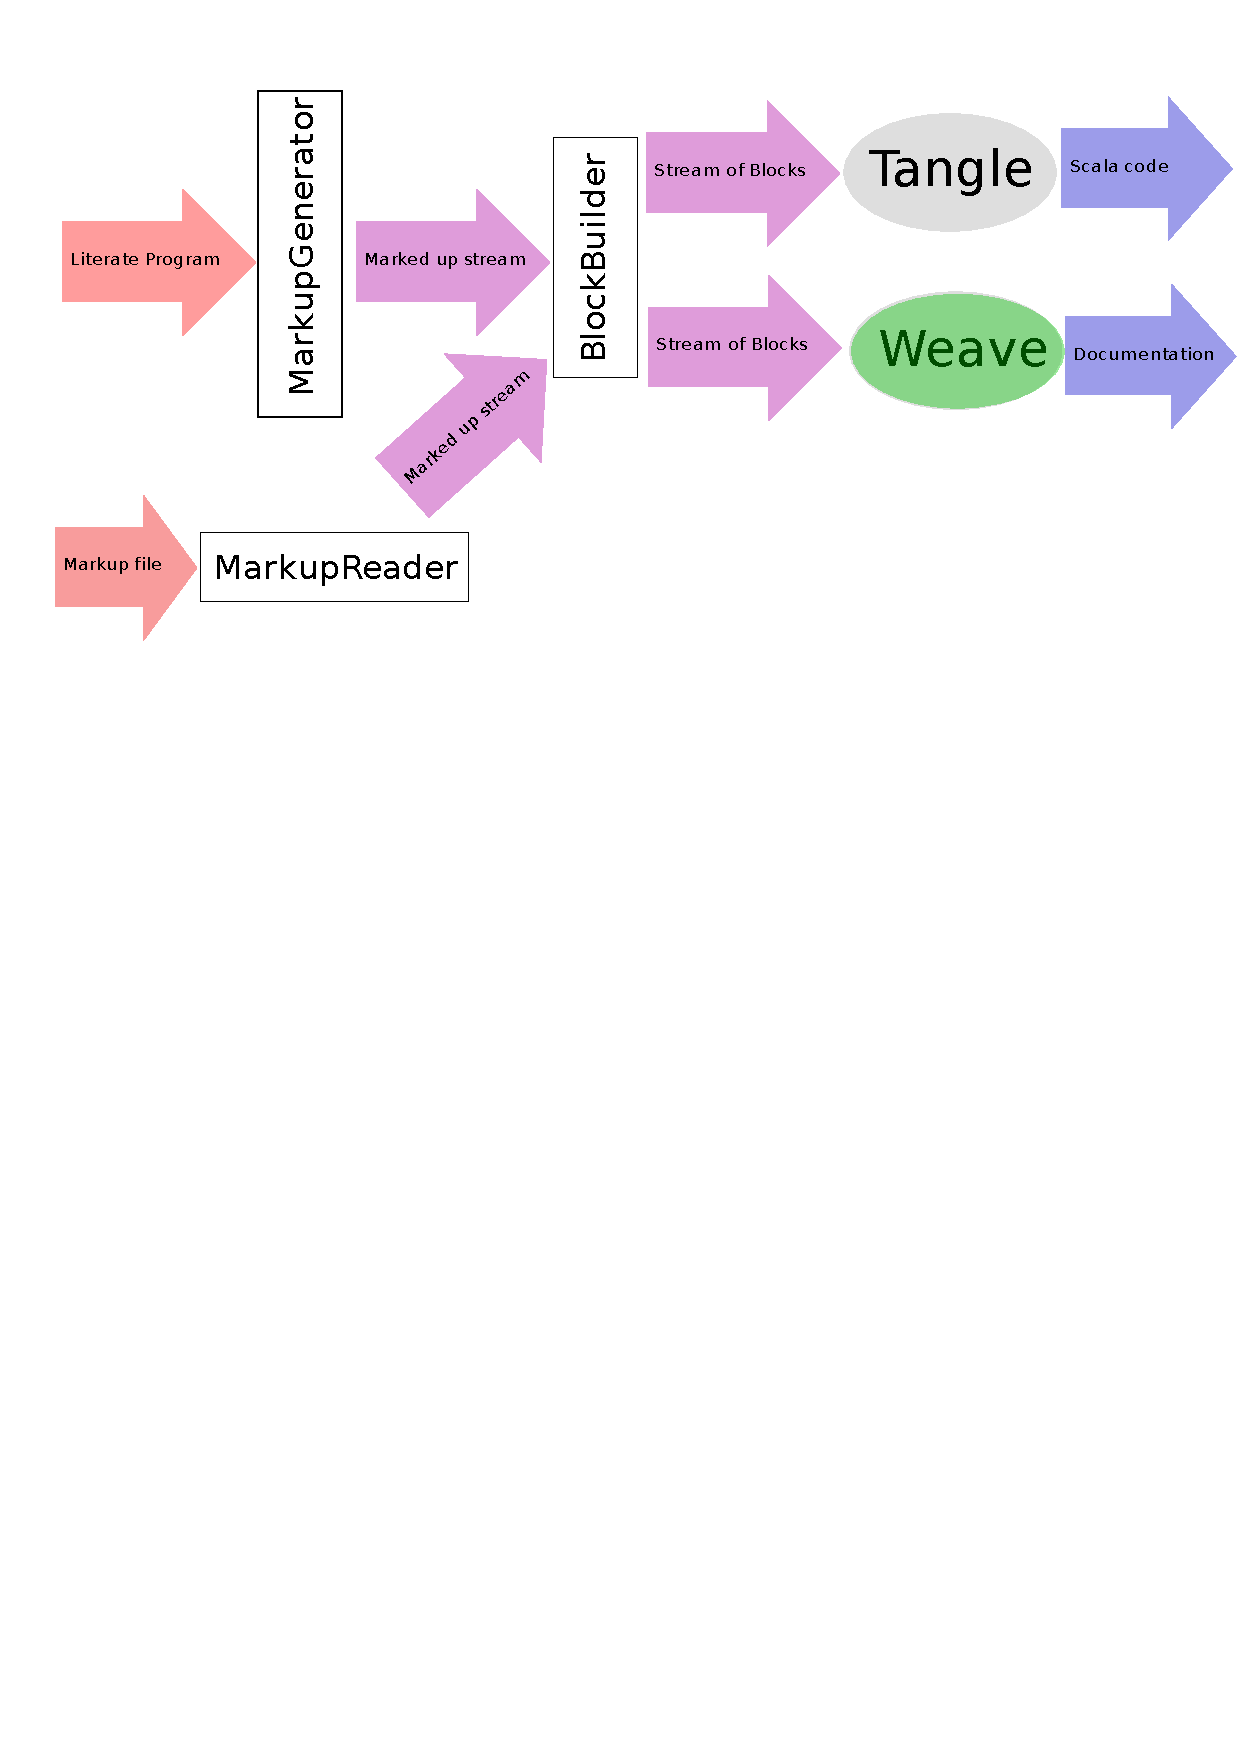
\includegraphics[width=10cm,viewport=310 610 600 710,clip]{images/weave}

It is important to note that there exists a tool to do syntactic
highlighting for scala called \texttt{verbfilter}\footnote{To be found under
misc/scala-tool-support/latex}. The method \texttt{process} takes a character
buffer and looks for \texttt{$\backslash$begin$\{$verbatim$\}$}, there it will begin to transform
the input. Our aim is therefore to convert the code sections to a character
buffer so that it can be fed to verbfilter.

$\left<\mbox{\emph{*}}\right>\equiv$
\begin{program}{\vem package}~scalit.weave
\\{\vem import}~markup.\_
\\[0.5em]$<$The~LaTeX~weaver$>$
\\[0.5em]$<$Source~file~information$>$
\\[0.5em]$<$The~command~line~application$>$
\\[0.5em]\end{program}


\subsection{The LaTeX weaver}
LatexWeaver, the class that takes care of producing LaTeX output from a list of
streams of blocks (as defined in \texttt{weave/blocks.nw}) has two methods: One for
printing one block, \texttt{printBlock}, and one to print everything surrounding
to produce a valid LaTeX document.

$\left<\mbox{\emph{The LaTeX weaver}}\right>\equiv$
\begin{program}{\vem sealed}~{\vem abstract}~{\vem class}~Weaver$($blocks\,{\rm :}~List$[$$($Stream$[$Block$]$,String$)$$]$$)$
\\[0.5em]{\vem case}~{\vem class}~LatexWeaver$($blocks\,{\rm :}~List$[$$($Stream$[$Block$]$,String$)$$]$,
\\~~~~~~~~~~~~~~~~~~~~~~~~~~~~~~tangled\,{\rm :}~List$[$tangle.ChunkCollection$]$,
\\~~~~~~~~~~~~~~~~~~~~~~~~~~~~~~useVerbfilter\,{\rm :}~Boolean,
\\~~~~~~~~~~~~~~~~~~~~~~~~~~~~~~useIndex\,{\rm :}~Boolean,
\\~~~~~~~~~~~~~~~~~~~~~~~~~~~~~~classpath\,{\rm :}~Option$[$List$[$String$]$$]$,
\\~~~~~~~~~~~~~~~~~~~~~~~~~~~~~~filename\,{\rm :}~String,
\\~~~~~~~~~~~~~~~~~~~~~~~~~~~~~~useHeader\,{\rm :}~Boolean$)$
\\~~~~~~~~~~{\vem extends}~Weaver$($blocks$)$~{\small\{}
\\[0.5em]~~~~{\vem import}~java.io.PrintStream
\\[0.5em]~~~~$<$escape~in~quoted~sections$>$
\\[0.5em]~~~~$<$escape~code$>$
\\[0.5em]~~~~$<$print~one~block$>$
\\[0.5em]~~~~$<$print~the~document$>$
\\[0.5em]~~~~$<$compiler~help$>$
\\[0.5em]~~~~$<$format~index$>$
\\{\small\}}
\\[0.5em]\end{program}\classdefinition{Weaver}
\classdefinition{LatexWeaver}
\valuedefinition{Weaver}{blocks}
\valuedefinition{LatexWeaver}{blocks }
\valuedefinition{LatexWeaver}{tangled }
\valuedefinition{LatexWeaver}{useVerbfilter }
\valuedefinition{LatexWeaver}{useIndex }
\valuedefinition{LatexWeaver}{classpath }
\valuedefinition{LatexWeaver}{filename }
\valuedefinition{LatexWeaver}{useHeader }



The useVerbfilter flag tells the weaver whether it should fire up the compiler
to retreive information on the source code. This is made optional because
it is pretty expensive. If \texttt{useHeader} is set to false, then we will not
print a header (ideal for inclusion in other LaTeX files).

\subsection{Printing one block}
There are two types of blocks to consider, code and documentation blocks. In
documentation blocks, we will need to know how to escape content: The backslash
character especially has to be escaped.

$\left<\mbox{\emph{escape in quoted sections}}\right>\equiv$
\begin{program}~~~~{\vem def}~escape$($orig\,{\rm :}~String$)${\rm :}~String~=~{\small\{}
\\~~~~~~~~orig.replace$($"$\backslash$$\backslash$","\Dollar$\backslash$$\backslash$backslash\Dollar"$)$
\\~~~~~~~~~~~~~~~~.replace$($"{\small\{}","\Dollar$\backslash$$\backslash${\small\{}\Dollar"$)$
\\~~~~~~~~~~~~~~~~.replace$($"{\small\}}","\Dollar$\backslash$$\backslash${\small\}}\Dollar"$)$
\\~~~~~~~~~~~~~~~~.replace$($"\#","\Dollar$\backslash$$\backslash$\#\Dollar"$)$
\\~~~~~~~~~~~~~~~~.replace$($"$<$","\Dollar$\backslash$$\backslash$langle\Dollar"$)$
\\~~~~~~~~~~~~~~~~.replace$($"$>$","\Dollar$\backslash$$\backslash$rangle\Dollar"$)$
\\~~~~~~~~~~~~~~~~.replace$($"\_","$\backslash$$\backslash$\_"$)$
\\~~~~{\small\}}
\\[0.5em]\end{program}\methoddefinition{LatexWeaver}{escape}



This function will undoubtedly be extended by more escape sequences. Now on
how to actually print these blocks. One speciality that we want to indicate
is whether we have already begun the definition of a given chunk. As this
would be too cumbersome to carry around, we'll keep track of it here:

$\left<\mbox{\emph{print one block}}\right>\equiv$
\begin{program}~~~~{\vem val}~chunksSeen~=
\\~~~~~~~~{\vem new}~scala.collection.mutable.HashMap$[$String,CodeBlock$]$
\\[0.5em]\end{program}


On to the block printing:

$\left<\mbox{\emph{print one block}}\right>+\equiv$
\begin{program}~~~~{\vem import}~StringRefs.\_
\\~~~~{\vem def}~printBlock$($out\,{\rm :}~PrintStream,
\\~~~~~~~~~~~~~~~~~~chunks\,{\rm :}~tangle.ChunkCollection$)$
\\~~~~~~~~~~~~~~~~~~$($b\,{\rm :}~Block$)${\rm :}~Unit~=~b~{\vem match}~{\small\{}
\\~~~~~~~~{\vem case}~cb~@~CodeBlock$($bn,ln,content,blockname$)$~$\Rightarrow$~{\small\{}
\\~~~~~~~~~~~~out.print$($"\Dollar$\backslash$$\backslash$left$<$$\backslash$$\backslash$mbox{\small\{}$\backslash$$\backslash$emph{\small\{}"~$+$
\\~~~~~~~~~~~~~~~~~~~~blockname~$+$
\\~~~~~~~~~~~~~~~~~~~~"{\small\}}{\small\}}$\backslash$$\backslash$right$>$"$)$
\\[0.5em]~~~~~~~~~~~~{\vem if}$($~chunksSeen~contains~blockname~$)$~out.print$($"$+$"$)$
\\~~~~~~~~~~~~{\vem else}~chunksSeen~$+$=~$($blockname~$\rightarrow$~cb~$)$
\\[0.5em]~~~~~~~~~~~~out.println$($"$\backslash$$\backslash$equiv\Dollar"$)$
\\[0.5em]\end{program}\methoddefinition{LatexWeaver}{printBlock}



Chunks that get defined for the first time start with
$\left<name\right>\equiv$, a continued chunk will be of the
form $\left<name\right>+\equiv$. If we use other code chunks,
this will be noted by $\left<name\right>$. In the following
section we will slurp the whole content of the code block
into a string:

$\left<\mbox{\emph{print one block}}\right>+\equiv$
\begin{program}~~~~~~~~~~~~{\vem var}~begin~=~$-$1
\\~~~~~~~~~~~~{\vem var}~end~~~=~$-$1
\\~~~~~~~~~~~~{\vem val}~content~=~"$\backslash$$\backslash$begin{\small\{}verbatim{\small\}}"~$+$
\\~~~~~~~~~~~~$($$($cb.stringRefForm$($chunks.cm$)$~map~{\small\{}
\\~~~~~~~~~~~~~~~~{\vem case}~RealString$($cont,from,to$)$~$\Rightarrow$~{\small\{}
\\~~~~~~~~~~~~~~~~~~~~{\vem if}$($~begin~$==$~$-$1~$)$~begin~=~from
\\[0.5em]~~~~~~~~~~~~~~~~~~~~{\vem if}$($~to~$>$~end~$)$~end~=~to
\\[0.5em]~~~~~~~~~~~~~~~~~~~~cont
\\~~~~~~~~~~~~~~~~{\small\}}
\\~~~~~~~~~~~~~~~~{\vem case}~BlockRef$($b$)$~$\Rightarrow$~{\small\{}
\\~~~~~~~~~~~~~~~~~~~~"$<$"~$+$
\\~~~~~~~~~~~~~~~~~~~~b.blockname~$+$
\\~~~~~~~~~~~~~~~~~~~~"$>$"
\\~~~~~~~~~~~~~~~~{\small\}}
\\~~~~~~~~~~~~~~~~{\vem case}~other~$\Rightarrow$~error$($"Unexpected\,{\rm :}~"~$+$~other$)$
\\~~~~~~~~~~~~{\small\}}~foldLeft~""$)$~{\small\{}
\\~~~~~~~~~~~~~~~~$($acc\,{\rm :}~String,~next\,{\rm :}~String$)$~$\Rightarrow$~acc~$+$~next
\\~~~~~~~~~~~~{\small\}}$)$~$+$~"$\backslash$$\backslash$"~$+$~"end{\small\{}verbatim{\small\}}"
\\[0.5em]\end{program}


If we want to use verbfilter, then we'll pass it to the script.
As we will have some unescaping to do (especially the $\Dollar$
character is troublesome) the output is not directly sent to
out but stored in a byte array, on which we can then apply the
unescaping. Also, if we want to create an index, we'll have to tell
it here.

$\left<\mbox{\emph{print one block}}\right>+\equiv$
\begin{program}~~~~{\vem if}$($~useVerbfilter~$)$~{\small\{}
\\~~~~~~~~{\vem val}~vfOutput~=~{\vem new}~java.io.ByteArrayOutputStream
\\~~~~~~~~toolsupport.verbfilterScala
\\~~~~~~~~~~~~.process$($codeEscape$($content$)$.getBytes,vfOutput$)$
\\~~~~~~~~{\vem if}$($~useIndex~$)$
\\~~~~~~~~~~~~out.println$($
\\~~~~~~~~~~~~~~~~indexed$($
\\~~~~~~~~~~~~~~~~codeUnescape$($
\\~~~~~~~~~~~~~~~~vfOutput.toString$)$,
\\~~~~~~~~~~~~~~~~begin,end,chunks.filename$)$$)$
\\~~~~~~~~{\vem else}
\\~~~~~~~~~~~~out.println$($codeUnescape$($vfOutput.toString$)$$)$
\\~~~~{\small\}}~{\vem else}~{\small\{}
\\~~~~~~~~{\vem if}$($~useIndex~$)$
\\~~~~~~~~~~~~out.println$($indexed$($content,
\\~~~~~~~~~~~~~~~~begin,end,chunks.filename$)$$)$
\\~~~~~~~~{\vem else}
\\~~~~~~~~~~~~out.println$($content$)$
\\~~~~{\small\}}
\\{\small\}}
\\[0.5em]\end{program}


Here we just avoided a quine-like problem: \texttt{$\backslash$end$\{$verbatim$\}$} is the sequence
to terminate a code block, so if it occurs inside a code block, then we could
run into a problem.

Documentation blocks will contain escaped sections (quoted), but otherwise
they will be copied verbatim.

$\left<\mbox{\emph{print one block}}\right>+\equiv$
\begin{program}~~~~~~~~{\vem case}~d~@~DocuBlock$($bn,ln,content$)$~$\Rightarrow$~{\small\{}
\\~~~~~~~~~~~~d.stringRefForm$($Map$($$)$$)$~foreach~{\small\{}
\\~~~~~~~~~~~~~~~~x~$\Rightarrow$~x~{\vem match}~{\small\{}
\\~~~~~~~~~~~~~~~~~~~~{\vem case}~RealString$($cont,\_,\_$)$~$\Rightarrow$~out.print$($cont$)$
\\~~~~~~~~~~~~~~~~~~~~{\vem case}~QuotedString$($cont$)$~$\Rightarrow$~{\small\{}
\\~~~~~~~~~~~~~~~~~~~~~~~~out.print$($"$\backslash$$\backslash$texttt{\small\{}"$)$
\\~~~~~~~~~~~~~~~~~~~~~~~~out.print$($escape$($cont$)$$)$
\\~~~~~~~~~~~~~~~~~~~~~~~~out.print$($"{\small\}}"$)$
\\~~~~~~~~~~~~~~~~~~~~{\small\}}
\\~~~~~~~~~~~~~~~~~~~~{\vem case}~BlockRef$($\_$)$~$\Rightarrow$
\\~~~~~~~~~~~~~~~~~~~~~~~~error$($"Did~not~expect~code~reference"~$+$
\\~~~~~~~~~~~~~~~~~~~~~~~~"~in~documentation~chunk"$)$
\\~~~~~~~~~~~~~~~~{\small\}}
\\~~~~~~~~~~~~{\small\}}
\\~~~~~~~~{\small\}}
\\~~~~{\small\}}
\\[0.5em]\end{program}


\subsubsection{Escaping code}
As we will pass code to the \texttt{verbfilter} program afterwards, we have to 
be very careful with some code content that could also be interpreted as
LaTeX escape sequences: We have to strip them out:

$\left<\mbox{\emph{escape code}}\right>\equiv$
\begin{program}~~~~{\vem def}~codeEscape$($code\,{\rm :}~String$)${\rm :}~String~=~{\small\{}
\\~~~~~~~~code.replace$($"\Dollar","SPEC"~$+$~"DOLLAR"$)$
\\~~~~{\small\}}
\\[0.5em]\end{program}\methoddefinition{LatexWeaver}{codeEscape}



The problem then is, of course, that we will need to put them back in
afterwards.

$\left<\mbox{\emph{escape code}}\right>+\equiv$
\begin{program}~~~~{\vem def}~codeUnescape$($code\,{\rm :}~String$)${\rm :}~String~=~{\small\{}
\\~~~~~~~~code.replace$($"SPEC"~$+$~"DOLLAR","$\backslash$$\backslash$Dollar"$)$
\\~~~~{\small\}}
\\[0.5em]\end{program}\methoddefinition{LatexWeaver}{codeUnescape}



\subsubsection{Wrapping the document}
With the knowledge on how to print blocks, we can go on printing the
whole document. If the useHeader flag is set (which it is by default),
we generate a standard LaTeX document, the only thing
special to note is that we add \texttt{scaladefs} which contains macros to
format scala output and \texttt{scalit} which enables definition indexing.

$\left<\mbox{\emph{print the document}}\right>\equiv$
\begin{program}~~~~{\vem def}~writeDoc$($out\,{\rm :}~PrintStream$)${\rm :}~Unit~=~{\small\{}
\\~~~~~~~~{\vem if}$($~useHeader~$)$~{\small\{}
\\~~~~~~~~~~~~out.println$($"$\backslash$$\backslash$documentclass$[$a4paper,12pt$]${\small\{}article{\small\}}"$)$
\\~~~~~~~~~~~~out.println$($"$\backslash$$\backslash$usepackage{\small\{}amsmath,amssymb{\small\}}"$)$
\\~~~~~~~~~~~~out.println$($"$\backslash$$\backslash$usepackage{\small\{}graphicx{\small\}}"$)$
\\~~~~~~~~~~~~out.println$($"$\backslash$$\backslash$usepackage{\small\{}scaladefs{\small\}}"$)$
\\~~~~~~~~~~~~out.println$($"$\backslash$$\backslash$usepackage{\small\{}scalit{\small\}}"$)$
\\~~~~~~~~~~~~out.println$($"$\backslash$$\backslash$usepackage{\small\{}fancyhdr{\small\}}"$)$
\\~~~~~~~~~~~~out.println$($"$\backslash$$\backslash$pagestyle{\small\{}fancy{\small\}}"$)$
\\~~~~~~~~~~~~out.println$($"$\backslash$$\backslash$lhead{\small\{}$\backslash$$\backslash$today{\small\}}"$)$
\\~~~~~~~~~~~~out.println$($"$\backslash$$\backslash$rhead{\small\{}"~$+$~escape$($filename$)$~$+$~"{\small\}}"$)$
\\~~~~~~~~~~~~out.println$($"$\backslash$$\backslash$begin{\small\{}document{\small\}}"$)$
\\~~~~~~~~{\small\}}
\\~~~~~~~~
\\~~~~~~~~blocks~zip~tangled~foreach~{\small\{}
\\~~~~~~~~~~~~{\vem case}~$($$($bs,\_$)$,tang$)$~$\Rightarrow$~bs~foreach~printBlock$($out,tang$)$
\\~~~~~~~~{\small\}}
\\[0.5em]~~~~~~~~{\vem if}$($~useHeader~$)$~{\small\{}
\\~~~~~~~~~~~~out.println$($"$\backslash$$\backslash$end{\small\{}document{\small\}}$\backslash$n$\backslash$n"$)$
\\~~~~~~~~{\small\}}
\\~~~~{\small\}}
\\[0.5em]\end{program}\methoddefinition{LatexWeaver}{writeDoc}



\subsection{Information on the source file}
During tangling, we directly interact with the compiler to compile from literate
programs. But the compiler can be of much more help - We can for example find
out where classes are defined, etc. For this, we reuse the source file class
defined for literate compilation\footnote{tangle/compilesupport.nw}.

Another optional parameter is where to find the classes containing
the other definitions: This will be used by the compiler to typecheck
the code, thus generating the symbols we need.

$\left<\mbox{\emph{Source file information}}\right>\equiv$
\begin{program}{\vem import}~scala.tools.nsc.ast.Trees
\\{\vem class}~SourceInformation$($
\\~~~~literateFile\,{\rm :}~tangle.LiterateProgramSourceFile,
\\~~~~infoClassPath\,{\rm :}~Option$[$List$[$String$]$$]$$)$~{\small\{}
\\~~~~$<$Instantiate~a~compiler$>$
\\[0.5em]~~~~$<$collect~information$>$
\\~~~~$<$range~of~definitions$>$
\\{\small\}}
\\[0.5em]$<$Definition~info~storage$>$
\\[0.5em]\end{program}\classdefinition{SourceInformation}
\valuedefinition{SourceInformation}{literateFile}
\valuedefinition{SourceInformation}{infoClassPath}



as with the compiler support class, we'll have to instantiate
a compiler. However, we will not need to do all the phases,
so we overwrite the phases we need:

$\left<\mbox{\emph{Instantiate a compiler}}\right>\equiv$
\begin{program}~~~~{\vem import}~scala.tools.nsc.{\small\{}Global,Settings,SubComponent{\small\}}
\\~~~~{\vem import}~scala.tools.nsc.reporters.ConsoleReporter
\\[0.5em]~~~~{\vem val}~settings~=~{\vem new}~Settings$($$)$
\\~~~~infoClassPath~{\vem match}~{\small\{}
\\~~~~~~~~{\vem case}~None~$\Rightarrow$~$($$)$
\\~~~~~~~~{\vem case}~Some$($cp$)$~$\Rightarrow$~settings.classpath.value~=~cp.head
\\~~~~{\small\}}
\\[0.5em]~~~~{\vem val}~reporter~=
\\~~~~~~~~{\vem new}~ConsoleReporter$($settings,{\vem null},
\\~~~~~~~~~~~~~~~~~~~~~~~~~~~~~~~~~~~~~~~~~~~~~~~~{\vem new}~java.io.PrintWriter$($System.err$)$$)$
\\~~~~{\vem object}~compiler~{\vem extends}~Global$($settings,~reporter$)$~{\small\{}
\\~~~~~~~~{\vem override}~{\vem protected}~{\vem def}~builtInPhaseDescriptors\,{\rm :}
\\~~~~~~~~List$[$SubComponent$]$~=~List$($
\\~~~~~~~~~~~~analyzer.namerFactory\,{\rm :}~SubComponent,
\\~~~~~~~~~~~~analyzer.typerFactory\,{\rm :}~SubComponent
\\~~~~~~~~$)$
\\~~~~{\small\}}
\\[0.5em]\end{program}\objectdefinition{compiler}
\methoddefinition{compiler}{builtInPhaseDescriptors}
\valuedefinition{SourceInformation}{settings }
\valuedefinition{SourceInformation}{reporter }



with the compiler in place, we can now define how to collect the information:

Execute the compiler just up to typing and collect them from the syntax tree.

$\left<\mbox{\emph{collect information}}\right>\equiv$
\begin{program}~~~~{\vem lazy}~{\vem val}~info~=~{\small\{}
\\~~~~~~~~{\vem val}~r~=~{\vem new}~compiler.Run
\\~~~~~~~~r.compileSources$($literateFile~{\rm :}{\rm :}~Nil$)$
\\[0.5em]~~~~~~~~{\vem val}~typedUnit~=~r.units.next
\\[0.5em]~~~~~~~~collectDefinitions$($typedUnit.body,Map$($$)$$)$
\\~~~~{\small\}}
\\[0.5em]\end{program}


The definition collector needs to have access to the tree case classes. They
are part of the compiler. We are very forgiving if, for example we do not find
a valid position.

$\left<\mbox{\emph{collect information}}\right>+\equiv$
\begin{program}~~~~{\vem import}~compiler.{\small\{}Tree,ClassDef,ModuleDef,PackageDef,
\\~~~~~~~~~~~~~~~~~~~~~~~~~~~~~~~~~~~~~~DefDef,ValDef,Template{\small\}}
\\~~~~{\vem import}~DefinitionInfo.\_
\\[0.5em]\end{program}


We will want to have access to the information on a per-line-basis. However,
there will be multiple definitions on one line, so we will need something like
a multiset:

$\left<\mbox{\emph{collect information}}\right>+\equiv$
\begin{program}~~~~{\vem type}~DefMap~=~Map$[$Int,Set$[$Definition$]$$]$
\\[0.5em]\end{program}


Another useful state to store is in which class we currently are, so that
we can link methods (which might be defined in multiple classes) to a specific
class. We overload this method to stay succinct.

$\left<\mbox{\emph{collect information}}\right>+\equiv$
\begin{program}~~~~{\vem def}~collectDefinitions$($t\,{\rm :}~Tree,~acc\,{\rm :}~DefMap$)${\rm :}~DefMap~=
\\~~~~~~~~collectDefinitions$($t,acc,None$)$
\\[0.5em]~~~~{\vem def}~collectDefinitions$($t\,{\rm :}~Tree,
\\~~~~~~~~~~~~~~~~~~~~~~~~~~~~~~~~~~acc\,{\rm :}~DefMap,
\\~~~~~~~~~~~~~~~~~~~~~~~~~~~~~~~~~~container\,{\rm :}~Option$[$String$]$$)${\rm :}~DefMap~=~{\small\{}
\\[0.5em]\end{program}\methoddefinition{SourceInformation}{collectDefinitions}
\methoddefinition{SourceInformation}{collectDefinitions}



After these overloaded definitions, let'l begin by getting the
source file position:

$\left<\mbox{\emph{collect information}}\right>+\equiv$
\begin{program}~~~~~~~~{\vem val}~pos~=~literateFile.positionInUltimateSource$($t.pos$)$
\\~~~~~~~~{\vem val}~line~=~pos.line~{\vem match}~{\small\{}
\\~~~~~~~~~~~~{\vem case}~None~$\Rightarrow$~$-$1
\\~~~~~~~~~~~~{\vem case}~Some$($l$)$~$\Rightarrow$~l
\\~~~~~~~~{\small\}}
\\~~~~~~~~{\vem val}~before~=~acc.getOrElse$($line,Set$($$)$$)$
\\~~~~~~~~t~{\vem match}~{\small\{}
\\$<$Handle~the~{\vem class}~{\vem case}$>$
\\$<$Handle~the~{\vem object}~{\vem case}$>$
\\$<$Handle~the~{\vem package}~{\vem case}$>$
\\$<$Handle~the~method~{\vem case}$>$
\\$<$Handle~the~value~{\vem case}$>$
\\~~~~~~~~~~~~{\vem case}~other~$\Rightarrow$~acc
\\~~~~~~~~{\small\}}
\\~~~~{\small\}}
\\[0.5em]\end{program}


The accumulator style makes this function rather heavy (note all the folds),
but this way we can append the definitions in a predictable style. So, on to the
starting point in our tree: The package definition

$\left<\mbox{\emph{Handle the package case}}\right>\equiv$
\begin{program}~~~~~~~~~~~~{\vem case}~PackageDef$($name,stats$)$~$\Rightarrow$
\\~~~~~~~~~~~~~~~~$($stats~foldLeft~acc$)$~{\small\{}
\\~~~~~~~~~~~~~~~~~~~~$($defs\,{\rm :}~DefMap,~t\,{\rm :}~Tree$)$~$\Rightarrow$~collectDefinitions$($t,defs$)$
\\~~~~~~~~~~~~~~~~{\small\}}
\\[0.5em]\end{program}


\texttt{defs} holds the current state of the map. Nodes of this package definition
will be classes and objects. We will first collect everything in the first class,
then pass the definition results to the second class, etc. Here is what we do with
classes:

$\left<\mbox{\emph{Handle the class case}}\right>\equiv$
\begin{program}{\vem case}~ClassDef$($\_,name,tparams,impl$)$~$\Rightarrow$
\\~~~~{\vem val}~nameString~=~name.toChars~mkString~""
\\~~~~{\vem val}~newAcc~=
\\~~~~~~~~acc~$+$~$($line~$\rightarrow$~$($before~$+$
\\~~~~~~~~~~~~~~~~~~~~~~~~~~~~~~~~~~~~~~~~ClassDefinition$($nameString,line,{\vem false}$)$$)$$)$
\\~~~~impl~{\vem match}~{\small\{}
\\~~~~~~~~{\vem case}~Template$($\_,\_,body$)$~$\Rightarrow$
\\~~~~~~~~~~~~$($body~foldLeft~newAcc$)$~{\small\{}
\\~~~~~~~~~~~~~~~~$($defs\,{\rm :}~DefMap,~t\,{\rm :}~Tree$)$~$\Rightarrow$
\\~~~~~~~~~~~~~~~~~~~~collectDefinitions$($t,defs,Some$($nameString$)$$)$
\\~~~~~~~~~~~~{\small\}}
\\~~~~{\small\}}
\\[0.5em]\end{program}


Classes have a body which we need to scan, but before we will have to add the class
itself to the map. If only that were so easy! Note that there are three basic types
of top-level objects on the class level:

\begin{itemize}
\item ``Normal'' classes
\item Objects
\item Case classes / objects
\end{itemize}

Note that this is not an either/or decision. A normal way to emulate static members in
Scala is the following:

\begin{verbatim}
class A {
  def aMethod = A.staticOne()
}
object A {
  def staticOne() = ...
}
\end{verbatim}

So we will be allowed to have object definitions and class definitions on different
lines. The compiler, however, seems to generate both \texttt{ClassDef} and \texttt{ModuleDef}
nodes when we have a case class. Also, the definition map is in an incomplete state,
so we can only bet on not seeing another \texttt{ClassDef} afterwards by assuming what
the compiler generates first the module definition element.
This first test tells us to only add contents if we are sure this actually is an
object. If we are dealing with a case class, we'll have to indicate this, for this
we will use the variable classDefinition.

$\left<\mbox{\emph{Do not add if object is there}}\right>\equiv$
\begin{program}~~~~~~~~~~~~~~~~{\vem var}~classDefinition\,{\rm :}~Option$[$ClassDefinition$]$~=~None
\\~~~~~~~~~~~~~~~~{\vem val}~isRealObject~=~acc~get~line~{\vem match}~{\small\{}
\\~~~~~~~~~~~~~~~~~~~~{\vem case}~Some$($s$)$~$\Rightarrow$~!$($s~exists~{\small\{}
\\~~~~~~~~~~~~~~~~~~~~~~~~{\vem case}~cd~@~ClassDefinition$($n,\_,\_$)$~$\Rightarrow$~{\small\{}
\\~~~~~~~~~~~~~~~~~~~~~~~~~~~~{\vem if}$($~n~$==$~nameString~$)$~{\small\{}
\\~~~~~~~~~~~~~~~~~~~~~~~~~~~~~~~~classDefinition~=~Some$($cd$)$
\\~~~~~~~~~~~~~~~~~~~~~~~~~~~~~~~~{\vem true}
\\~~~~~~~~~~~~~~~~~~~~~~~~~~~~{\small\}}~{\vem else}~{\vem false}
\\~~~~~~~~~~~~~~~~~~~~~~~~{\small\}}
\\~~~~~~~~~~~~~~~~~~~~~~~~{\vem case}~other~$\Rightarrow$~{\vem false}
\\~~~~~~~~~~~~~~~~~~~~{\small\}}$)$
\\~~~~~~~~~~~~~~~~~~~~{\vem case}~None~$\Rightarrow$~~~~~~~~~{\vem true}
\\~~~~~~~~~~~~~~~~{\small\}}
\\[0.5em]\end{program}


If we have already content on this line, then we will not traverse it again, but
we will update the fact that we are dealing with a case class.

$\left<\mbox{\emph{Handle the object case}}\right>\equiv$
\begin{program}{\vem case}~ModuleDef$($mods,name,impl$)$~$\Rightarrow$
\\~~~~{\vem val}~nameString~=~name.toChars~mkString~""
\\~~~~$<$Do~not~add~{\vem if}~{\vem object}~is~there$>$
\\~~~~{\vem if}$($isRealObject$)$~{\small\{}
\\~~~~~~~~{\vem val}~newAcc~=~acc~$+$~$($line~$\rightarrow$
\\~~~~~~~~~~~~~~~~$($before~$+$~ObjectDefinition$($nameString,line$)$$)$$)$
\\~~~~~~~~impl~{\vem match}~{\small\{}
\\~~~~~~~~~~~~{\vem case}~Template$($\_,\_,body$)$~$\Rightarrow$
\\~~~~~~~~~~~~~~~~$($body~foldLeft~newAcc$)$~{\small\{}
\\~~~~~~~~~~~~~~~~~~~~$($defs\,{\rm :}~DefMap,~t\,{\rm :}~Tree$)$~$\Rightarrow$
\\~~~~~~~~~~~~~~~~~~~~~~~~collectDefinitions$($t,defs,Some$($nameString$)$$)$
\\~~~~~~~~~~~~~~~~{\small\}}
\\~~~~~~~~{\small\}}
\\~~~~{\small\}}~{\vem else}~{\small\{}
\\~~~~~~~~{\vem val}~Some$($cd$)$~=~classDefinition
\\~~~~~~~~{\vem val}~cc~=~ClassDefinition$($cd.name,cd.l,{\vem true}$)$
\\~~~~~~~~acc~$+$~$($line~$\rightarrow$~$($before~$-$~cd~$+$~cc$)$$)$
\\~~~~{\small\}}
\\[0.5em]\end{program}


For the definitions, We will have to use the same trick as for objects: Some
methods are added automatically (like toString, <init>) and should therefore not
be included in the index. We solve this by looking up whether a class was defined
on the same line. Also, it might be that there exists already a value definition with
the same name, in which case we won't add it either:

$\left<\mbox{\emph{Handle the method case}}\right>\equiv$
\begin{program}{\vem case}~DefDef$($\_,name,tparams,vparams,tpt,\_$)$~$\Rightarrow$
\\~~~~{\vem val}~isGeneratedMethod~=~acc~get~line~{\vem match}~{\small\{}
\\~~~~~~~~{\vem case}~None~$\Rightarrow$~{\vem false}
\\~~~~~~~~{\vem case}~Some$($s$)$~$\Rightarrow$~s~exists~{\small\{}
\\~~~~~~~~~~~~{\vem case}~c~{\rm :}~ClassDefinition~$\Rightarrow$~{\vem true}
\\~~~~~~~~~~~~{\vem case}~o~{\rm :}~ObjectDefinition~$\Rightarrow$~{\vem true}
\\~~~~~~~~~~~~{\vem case}~vd~{\rm :}~ValueDefinition~$\Rightarrow$~{\vem true}
\\~~~~~~~~~~~~{\vem case}~\_~$\Rightarrow$~{\vem false}
\\~~~~~~~~{\small\}}
\\~~~~{\small\}}
\\~~~~{\vem if}$($~isGeneratedMethod~$)$~acc
\\~~~~{\vem else}~acc~$+$~$($line~$\rightarrow$
\\~~~~~~~~$($before~$+$~MethodDefinition$($name.toString,line,container$)$$)$$)$
\\[0.5em]\end{program}


We also record value definitions

$\left<\mbox{\emph{Handle the value case}}\right>\equiv$
\begin{program}~~~~~~~~~~~~{\vem case}~ValDef$($\_,name,\_,\_$)$~$\Rightarrow$~{\small\{}
\\~~~~~~~~~~~~~~~~{\vem val}~nameString~=~name.toChars~mkString~""
\\~~~~~~~~~~~~~~~~acc~$+$~$($line~$\rightarrow$~$($before~$+$~ValueDefinition$($nameString,line,container$)$$)$$)$~
\\~~~~~~~~~~~~{\small\}}
\\[0.5em]\end{program}


 One useful
command would be to get all the definitions in a range of lines:

$\left<\mbox{\emph{range of definitions}}\right>\equiv$
\begin{program}~~~~{\vem def}~getRange$($from\,{\rm :}~Int,~to\,{\rm :}~Int$)${\rm :}~List$[$Definition$]$~=
\\~~~~~~~~List.range$($from,to~$+$~1$)$~flatMap~{\small\{}
\\~~~~~~~~~~~~i~$\Rightarrow$~info.getOrElse$($i,Nil$)$
\\~~~~~~~~{\small\}}
\\[0.5em]\end{program}\methoddefinition{SourceInformation}{getRange}



\subsubsection{Connection to the weaver}
Especially in LaTeXWeaver, we will want to auto-generate some annotations,
therefore we'll have to have a value for that:

$\left<\mbox{\emph{compiler help}}\right>\equiv$
\begin{program}~~~~{\vem import}~tangle.LiterateProgramSourceFile
\\~~~~{\vem val}~sourcefiles\,{\rm :}~Option$[$List$[$$($String,LiterateProgramSourceFile$)$$]$$]$~=
\\~~~~~~~~{\vem if}$($~useIndex~$)$~{\small\{}
\\~~~~~~~~~~~~Some$($tangled~map~{\small\{}
\\~~~~~~~~~~~~~~~~chunks~$\Rightarrow$
\\~~~~~~~~~~~~~~~~~~~~$($chunks.filename,
\\~~~~~~~~~~~~~~~~~~~~~~{\vem new}~tangle.LiterateProgramSourceFile$($chunks$)$$)$
\\~~~~~~~~~~~~{\small\}}$)$
\\~~~~~~~~{\small\}}~{\vem else}~None
\\[0.5em]~~~~{\vem val}~sourceInformation\,{\rm :}~Map$[$String,SourceInformation$]$~=
\\~~~~sourcefiles~{\vem match}~{\small\{}
\\~~~~~~~~{\vem case}~None~$\Rightarrow$~Map$($$)$
\\~~~~~~~~{\vem case}~Some$($sfs$)$~$\Rightarrow$~Map$($$)$~$+$$+$~$($sfs~map~{\small\{}
\\~~~~~~~~~~~~{\vem case}~$($name,sf$)$~$\Rightarrow$~$($name~$\rightarrow$~{\vem new}~SourceInformation$($sf,classpath$)$$)$
\\~~~~~~~~{\small\}}$)$
\\~~~~{\small\}}
\\[0.5em]\end{program}


\subsubsection{Storing the gathered information}
While traversing the tree, we need to store information on what is actually
defined. This is particularly:

\begin{itemize}
\item Class and trait definitions
\item Object definitions
\item Method definitions
\end{itemize}

To each element, we'll want to store the line number so that it can be easily
retrieved.

$\left<\mbox{\emph{Definition info storage}}\right>\equiv$
\begin{program}{\vem object}~DefinitionInfo~{\small\{}
\\~~~~{\vem sealed}~{\vem abstract}~{\vem class}~Definition$($line\,{\rm :}~Int$)$
\\[0.5em]~~~~{\vem case}~{\vem class}~ClassDefinition$($name\,{\rm :}~String,~l\,{\rm :}~Int,
\\~~~~~~~~~~~~~~~~~~~~~~~~~~~~~~~~~~~~~~~~~~~~~~~~~~isCase\,{\rm :}~Boolean$)$
\\~~~~~~~~{\vem extends}~Definition$($l$)$~{\small\{}
\\~~~~~~~~~~~~{\vem override}~{\vem def}~toString~=~""~$+$~l~$+$~"{\rm :}~Class~"~$+$~name
\\~~~~~~~~{\small\}}
\\[0.5em]~~~~{\vem case}~{\vem class}~ObjectDefinition$($name\,{\rm :}~String,
\\~~~~~~~~~~~~~~~~~~~~~~~~~~~~~~~~~~~~~~~~~~~~~~~~~~l\,{\rm :}~Int$)$
\\~~~~~~~~{\vem extends}~Definition$($l$)$~{\small\{}
\\~~~~~~~~~~~~{\vem override}~{\vem def}~toString~=~""~$+$~l~$+$~"{\rm :}~Object~"~$+$~name
\\~~~~~~~~{\small\}}
\\[0.5em]~~~~{\vem case}~{\vem class}~MethodDefinition$($name\,{\rm :}~String,
\\~~~~~~~~~~~~~~~~~~~~~~~~~~~~~~~~~~~~~~~~~~~~~~~~~~l\,{\rm :}~Int,
\\~~~~~~~~~~~~~~~~~~~~~~~~~~~~~~~~~~~~~~~~~~~~~~~~~~container\,{\rm :}~Option$[$String$]$$)$
\\~~~~~~~~{\vem extends}~Definition$($l$)$~{\small\{}
\\~~~~~~~~~~~~{\vem override}~{\vem def}~toString~=~""~$+$~l~$+$~"{\rm :}~Method~"~$+$~name
\\~~~~~~~~{\small\}}
\\[0.5em]~~~~{\vem case}~{\vem class}~ValueDefinition$($name\,{\rm :}~String,
\\~~~~~~~~~~~~~~~~~~~~~~~~~~~~~~~~~~~~~~~~~~~~~~~~~~l\,{\rm :}~Int,
\\~~~~~~~~~~~~~~~~~~~~~~~~~~~~~~~~~~~~~~~~~~~~~~~~~~container\,{\rm :}~Option$[$String$]$$)$
\\~~~~~~~~{\vem extends}~Definition$($l$)$~{\small\{}
\\~~~~~~~~~~~~{\vem override}~{\vem def}~toString~=~""~$+$~l~$+$~"{\rm :}~Value~"~$+$~name
\\~~~~~~~~{\small\}}
\\{\small\}}
\\[0.5em]\end{program}\classdefinition{Definition}
\classdefinition{ClassDefinition}
\classdefinition{ObjectDefinition}
\classdefinition{MethodDefinition}
\classdefinition{ValueDefinition}
\objectdefinition{DefinitionInfo}
\methoddefinition{ClassDefinition}{toString}
\methoddefinition{ObjectDefinition}{toString}
\methoddefinition{MethodDefinition}{toString}
\methoddefinition{ValueDefinition}{toString}
\valuedefinition{Definition}{line}
\valuedefinition{ClassDefinition}{name }
\valuedefinition{ClassDefinition}{l }
\valuedefinition{ClassDefinition}{isCase }
\valuedefinition{ObjectDefinition}{name }
\valuedefinition{ObjectDefinition}{l }
\valuedefinition{MethodDefinition}{name }
\valuedefinition{MethodDefinition}{l }
\valuedefinition{MethodDefinition}{container }
\valuedefinition{ValueDefinition}{name }
\valuedefinition{ValueDefinition}{l }
\valuedefinition{ValueDefinition}{container }



\subsubsection{Testing the information gathering}
The following command line tool tests the information gathering:

$\left<\mbox{\emph{Source file information}}\right>+\equiv$
\begin{program}{\vem object}~InfoTester~{\small\{}
\\~~~~{\vem def}~main$($args\,{\rm :}~Array$[$String$]$$)$~=~{\small\{}
\\~~~~~~~~{\vem import}~util.LiterateSettings
\\~~~~~~~~{\vem import}~tangle.LiterateProgramSourceFile
\\[0.5em]
\\~~~~~~~~{\vem val}~ls~=~{\vem new}~LiterateSettings$($args$)$
\\[0.5em]~~~~~~~~{\vem val}~sourceFiles~=
\\~~~~~~~~~~~~ls.chunkCollections~map~$($
\\~~~~~~~~~~~~~~~~{\vem new}~LiterateProgramSourceFile$($\_$)$$)$
\\[0.5em]~~~~~~~~{\vem val}~infoclasspath~=~ls.settings~get~"$-$classpath"
\\[0.5em]~~~~~~~~{\vem val}~infolist~=
\\~~~~~~~~~~~~sourceFiles~map~$(${\vem new}~SourceInformation$($\_,infoclasspath$)$$)$
\\[0.5em]~~~~~~~~infolist~foreach~{\small\{}~x~$\Rightarrow$~println$($x.getRange$($0,50$)$$)$~{\small\}}
\\~~~~{\small\}}
\\{\small\}}
\\[0.5em]\end{program}\objectdefinition{InfoTester}
\methoddefinition{InfoTester}{main}



\subsubsection{Adding index information}
With the compiler support that we defined before, we will be able to print
which functions were defined in a piece of code. The following function adds
these bits:

$\left<\mbox{\emph{format index}}\right>\equiv$
\begin{program}~~~~{\vem def}~indexed$($content\,{\rm :}~String,~from\,{\rm :}~Int,
\\~~~~~~~~~~~~~~~~~~~~~~~~~~~~to\,{\rm :}~Int,~filename\,{\rm :}~String$)${\rm :}~String~=~{\small\{}
\\~~~~~~~~{\vem import}~DefinitionInfo.\_
\\~~~~~~~~{\vem val}~ret~=~{\vem new}~StringBuffer
\\~~~~~~~~ret~append~content
\\~~~~~~~~
\\~~~~~~~~sourceInformation~get~filename~{\vem match}~{\small\{}
\\~~~~~~~~~~~~{\vem case}~None~$\Rightarrow$~$($$)$
\\~~~~~~~~~~~~{\vem case}~Some$($si$)$~$\Rightarrow$~{\small\{}
\\~~~~~~~~~~~~~~~~{\vem val}~definitions~=~si.getRange$($from,to$)$
\\[0.5em]\end{program}\methoddefinition{LatexWeaver}{indexed}



The first definitions that we are interested in are which classes
are defined:

$\left<\mbox{\emph{format index}}\right>+\equiv$
\begin{program}~~~~~~~~~~~~~~~~{\vem val}~classes~=~definitions~filter~{\small\{}
\\~~~~~~~~~~~~~~~~~~~~{\vem case}~cd\,{\rm :}~ClassDefinition~$\Rightarrow$~{\vem true}
\\~~~~~~~~~~~~~~~~~~~~{\vem case}~\_~$\Rightarrow$~{\vem false}
\\~~~~~~~~~~~~~~~~{\small\}}
\\[0.5em]\end{program}


Then methods. Here, we want to filter out the generated methods

$\left<\mbox{\emph{format index}}\right>+\equiv$
\begin{program}~~~~~~~~~~~~~~~~{\vem val}~methods~=~definitions~filter~{\small\{}
\\~~~~~~~~~~~~~~~~~~~~{\vem case}~MethodDefinition$($name,\_,\_$)$~$\Rightarrow$~{\vem true}
\\~~~~~~~~~~~~~~~~~~~~{\vem case}~\_~$\Rightarrow$~{\vem false}
\\~~~~~~~~~~~~~~~~{\small\}}
\\[0.5em]\end{program}


Values and objects are filtered in a same way

$\left<\mbox{\emph{format index}}\right>+\equiv$
\begin{program}~~~~~~~~~~~~~~~~{\vem val}~values~=~definitions~filter~{\small\{}
\\~~~~~~~~~~~~~~~~~~~~{\vem case}~v~{\rm :}~ValueDefinition~$\Rightarrow$~{\vem true}
\\~~~~~~~~~~~~~~~~~~~~{\vem case}~\_~$\Rightarrow$~{\vem false}
\\~~~~~~~~~~~~~~~~{\small\}}
\\~~~~~~~~~~~~~~~~{\vem val}~objects~=~definitions~filter~{\small\{}
\\~~~~~~~~~~~~~~~~~~~~{\vem case}~o\,{\rm :}~ObjectDefinition~$\Rightarrow$~{\vem true}
\\~~~~~~~~~~~~~~~~~~~~{\vem case}~\_~$\Rightarrow$~{\vem false}
\\~~~~~~~~~~~~~~~~{\small\}}
\\[0.5em]\end{program}


Now for the LaTeX output generated: We use the commands defined
in \texttt{scalit.sty} so that we can change presentation later on. Note that
no real output needs to be generated.

$\left<\mbox{\emph{format index}}\right>+\equiv$
\begin{program}~~~~~~~~~~~~~~~~{\vem if}~$($!classes.isEmpty~$\,|$$\,|$~!methods.isEmpty~$\,|$$\,|$
\\~~~~~~~~~~~~~~~~~~~~~~~~!objects.isEmpty$)$~{\small\{}
\\$<$output~{\vem class}~definition~info$>$
\\$<$output~{\vem object}~definition~info$>$
\\$<$output~method~definition~info$>$
\\$<$output~value~definition~info$>$
\\~~~~~~~~~~~~~~~~{\small\}}
\\~~~~~~~~~~~~~~~~ret~append~"$\backslash$n$\backslash$n"
\\~~~~~~~~~~~~{\small\}}
\\~~~~~~~~{\small\}}
\\[0.5em]~~~~~~~~ret.toString
\\~~~~{\small\}}
\\[0.5em]\end{program}


First the classes. The command \texttt{classdefinition} takes care
of them. At the moment, we are not indicating case classes specially.

$\left<\mbox{\emph{output class definition info}}\right>\equiv$
\begin{program}classes~foreach~{\small\{}
\\~~~~{\vem case}~ClassDefinition$($name,\_,caseClass$)$~$\Rightarrow$~{\small\{}
\\~~~~~~~~ret~append~"$\backslash$$\backslash$classdefinition{\small\{}"~$+$~name~$+$~"{\small\}}$\backslash$n"
\\~~~~{\small\}}
\\~~~~{\vem case}~\_~$\Rightarrow$~$($$)$
\\{\small\}}
\\[0.5em]\end{program}


Second come the object definitions.

$\left<\mbox{\emph{output object definition info}}\right>\equiv$
\begin{program}objects~foreach~{\small\{}
\\~~~~{\vem case}~ObjectDefinition$($name,\_$)$~$\Rightarrow$~{\small\{}
\\~~~~~~~~ret~append~"$\backslash$$\backslash$objectdefinition{\small\{}"~$+$~name~$+$~"{\small\}}$\backslash$n"
\\~~~~{\small\}}
\\~~~~{\vem case}~\_~$\Rightarrow$~$($$)$
\\{\small\}}
\\[0.5em]\end{program}


Methods are prefixed by the class in which they are defined. Note
the flaw in this system: This way we are only recording one level
of classes, thus generating a flat index. Also, the body of the
methods is not further traversed, so inner functions are not
detected.

$\left<\mbox{\emph{output method definition info}}\right>\equiv$
\begin{program}methods~foreach~{\small\{}
\\~~~~{\vem case}~MethodDefinition$($name,\_,cont$)$~$\Rightarrow$~{\small\{}
\\~~~~~~~~ret~append~"$\backslash$$\backslash$methoddefinition{\small\{}"
\\~~~~~~~~cont~{\vem match}~{\small\{}
\\~~~~~~~~~~~~{\vem case}~None~$\Rightarrow$~$($$)$
\\~~~~~~~~~~~~~~~~{\vem case}~Some$($n$)$~$\Rightarrow$~ret~append~escape$($n$)$
\\~~~~~~~~{\small\}}
\\~~~~~~~~ret~append~"{\small\}}{\small\{}"
\\~~~~~~~~ret~append~escape$($name$)$~$+$~"{\small\}}$\backslash$n"
\\~~~~{\small\}}
\\~~~~{\vem case}~\_~$\Rightarrow$~$($$)$
\\{\small\}}
\\[0.5em]\end{program}


Value definitions are also noted. This might be a bit
overkill, so in a further stage we could filter for only
publicly accessible values.

$\left<\mbox{\emph{output value definition info}}\right>\equiv$
\begin{program}values~foreach~{\small\{}
\\~~~~{\vem case}~ValueDefinition$($name,\_,cont$)$~$\Rightarrow$~{\small\{}
\\~~~~~~~~ret~append~"$\backslash$$\backslash$valuedefinition{\small\{}"
\\~~~~~~~~cont~{\vem match}~{\small\{}
\\~~~~~~~~~~~~{\vem case}~None~$\Rightarrow$~$($$)$
\\~~~~~~~~~~~~~~~~{\vem case}~Some$($n$)$~$\Rightarrow$~ret~append~escape$($n$)$
\\~~~~~~~~{\small\}}
\\~~~~~~~~ret~append~"{\small\}}{\small\{}"
\\~~~~~~~~ret~append~name~$+$~"{\small\}}$\backslash$n"
\\~~~~{\small\}}
\\~~~~{\vem case}~\_~$\Rightarrow$~$($$)$
\\{\small\}}
\\[0.5em]\end{program}


\subsection{The command line application}
The command line application gets quite a bit more complicated than before:
Not only do we scan the code blocks but we also tangle the source! This way
we can assure that we do not reference code blocks in the text that were not
defined. Also, in a later stage we could use compiler information to see
what is defined where etc. \texttt{LiterateSettings}\footnote{See util/commandline.nw}
lets us read in multiple files
to form one LaTeX document.

Specifically, it takes the following options:

\begin{description}
\item[-vf t/f] if t, then apply verbfilter on source. Default true
\item[-idx t/f] if t, then generate definition index. Default false
\item[-classpath path] Classpath to be used for reference to other
classes if index is built.
\end{description}

$\left<\mbox{\emph{The command line application}}\right>\equiv$
\begin{program}{\vem object}~Weave~{\small\{}
\\~~~~{\vem def}~main$($args\,{\rm :}~Array$[$String$]$$)$~=~{\small\{}
\\~~~~~~~~{\vem import}~util.LiterateSettings
\\[0.5em]~~~~~~~~{\vem val}~ls~=~{\vem new}~LiterateSettings$($args$)$
\\[0.5em]~~~~~~~~{\vem val}~blocks~{\rm :}~List$[$$($Stream$[$markup.Block$]$,String$)$$]$~=~ls.blocks
\\[0.5em]\end{program}\objectdefinition{Weave}
\methoddefinition{Weave}{main}



This is the same as with tangle: We want to extract
code blocks from the line format. We will actually
partially execute the tangle phase: The part where we
put chunks together.

But first, let us deal with the title of the file. If one is specified
on the command line, we use this. Otherwise, we use the name of the first
file given as input.

$\left<\mbox{\emph{The command line application}}\right>+\equiv$
\begin{program}~~~~~~~~{\vem val}~filename~=~ls.settings~get~"$-$title"~{\vem match}~{\small\{}
\\~~~~~~~~~~~~{\vem case}~Some$($x\,{\rm :}{\rm :}xs$)$~$\Rightarrow$~x
\\~~~~~~~~~~~~{\vem case}~\_~$\Rightarrow$~blocks~{\vem match}~{\small\{}
\\~~~~~~~~~~~~~~~~{\vem case}~$($\_,name$)$~{\rm :}{\rm :}~xs~$\Rightarrow$~name
\\~~~~~~~~~~~~~~~~{\vem case}~Nil~$\Rightarrow$~""
\\~~~~~~~~~~~~{\small\}}
\\~~~~~~~~{\small\}}
\\[0.5em]\end{program}


Some settings are taken out of the settings object directly,
where to send output is handled specially.

$\left<\mbox{\emph{The command line application}}\right>+\equiv$
\begin{program}~~~~~~~~{\vem val}~classpath~=~ls.settings~get~"$-$classpath"
\\[0.5em]~~~~~~~~{\vem val}~verbfilter~=~ls.settings~get~"$-$vf"~{\vem match}~{\small\{}
\\~~~~~~~~~~~~{\vem case}~Some$($x~{\rm :}{\rm :}~xs$)$~$\Rightarrow$~x$($0$)$~$==$~'t'
\\~~~~~~~~~~~~{\vem case}~\_~$\Rightarrow$~{\vem true}
\\~~~~~~~~{\small\}}
\\[0.5em]~~~~~~~~{\vem val}~index~=~ls.settings~get~"$-$idx"~{\vem match}~{\small\{}
\\~~~~~~~~~~~~{\vem case}~Some$($x~{\rm :}{\rm :}~xs$)$~$\Rightarrow$~x$($0$)$~$==$~'t'
\\~~~~~~~~~~~~{\vem case}~\_~$\Rightarrow$~{\vem false}
\\~~~~~~~~{\small\}}
\\[0.5em]\end{program}


This follows a very general pattern: If the option does not exist, it
gets a default value, otherwise it depends on the option whether we interpret
it as truth value or otherwise. The following option is on whether to include
a header in the generated \texttt{tex} file. By default, we print one:

$\left<\mbox{\emph{The command line application}}\right>+\equiv$
\begin{program}~~~~~~~~{\vem val}~header~=~ls.settings~get~"$-$header"~{\vem match}~{\small\{}
\\~~~~~~~~~~~~{\vem case}~Some$($x~{\rm :}{\rm :}~xs$)$~$\Rightarrow$~x$($0$)$~$==$~'t'
\\~~~~~~~~~~~~{\vem case}~\_~$\Rightarrow$~{\vem true}
\\~~~~~~~~{\small\}}
\\[0.5em]~~~~~~~~{\vem val}~weaved~=~LatexWeaver$($blocks,ls.chunkCollections,
\\~~~~~~~~~~~~~~~~~~~~~~~~~~~~~~~~~~~~~~~~~~verbfilter,index,classpath,filename,
\\~~~~~~~~~~~~~~~~~~~~~~~~~~~~~~~~~~~~~~~~~~header$)$
\\[0.5em]~~~~~~~~weaved.writeDoc$($ls.output$)$
\\~~~~{\small\}}
\\{\small\}}
\\[0.5em]\end{program}


 \pagebreak

\classindex
\end{document}


